\chapter[Synthesis]{Synthesis}
In this chapter of the report, the theory discussed in the previous chapter will be applied to synthesise the design parameters of the class-D amplifier. The initial design parameters can be seen in \autoref{tab:initial_design_parameters}.

\begin{table}[htbp]
	\centering
	\begin{tabular}{@{}llll@{}}
		\toprule
		\multicolumn{1}{c}{\textbf{Name}} & \textbf{Value}        & \textbf{Unit}         & \textbf{Description} \\ \midrule
		$V_{\mathrm{sup}}$ & $5$ & \si{\volt} & Low-voltage supply \\
		$V_{\mathrm{DD}}$  & $30$  & \si{\volt}   & Power supply      \\
		$V_{\mathrm{ref}}$ & $2.5$ & \si{\volt}   & Reference voltage \\
		$R_\mathrm{{BTL}}$ & $4$   & \si{\ohm} & Bridge-tied load \\ \bottomrule
	\end{tabular}
	\caption{Initial design parameters of the amplifier}
	\label{tab:initial_design_parameters}
\end{table}

Through each section of this chapter, the methodology of calculating component values to the various sub-circuits will be explained.

\section{Preamplifier and Input Filter}
As mentioned in \autoref{sec:theory_filter_preamp} the circuit will be designed with a high-pass and a low-pass filter in mind. The result is a bandpass filter. The methodology here will be choosing a capacitor value and dimensioning the resistive component based on the expression.

\begin{table}[htbp]
	\centering
	\begin{tabular}{@{}llll@{}}
		\toprule
		\multicolumn{1}{c}{\textbf{Name}} & \textbf{Value} & \textbf{Unit} & \textbf{Description} \\ \midrule
		$f_{\mathrm{hp}}$ & $10$ & \si{\hertz} & High-pass cut-off frequency \\
		$f_{\mathrm{lp}}$ & $80$ & \si{\kilo\hertz} & Low-pass cut-off frequency \\
		$C_{\mathrm{1}}$ & $1$  & \si{\micro\farad}  & High-pass filter capacitor \\
		$C_{\mathrm{2}}$ & $1$  & \si{\nano\farad}  & Low-pass filter capacitor  \\
		$A_{v}$  & $2$  & $1$   & Gain                       \\ \bottomrule
	\end{tabular}
	\caption{Initial design parameters of the preamp and filter}
	\label{tab:design_parameters_preamp_filter}
\end{table}
As the two capacitive components are now decided, the values from \autoref{tab:design_parameters_preamp_filter} are now input in \Cref{eq:preamp_cut-off-filtersa,eq:preamp_cut-off-filtersb}.
\begin{subequations} \label{eq:preamp_cut-off_synth}
	\begin{equation} \label{eq:preamp_cut-off_synth_a}
		R_{1} = \frac{1}{2\pi \cdot \SI{10}{\hertz} \cdot \SI{1}{\micro\farad}} = \SI{15.92}{\kilo\ohm}
	\end{equation}
	\begin{equation} \label{eq:preamp_cut-off_synth_b}
		R_{2} = \frac{1}{2\pi \cdot \SI{80}{\kilo\hertz} \cdot \SI{1}{\nano\farad}} = \SI{1.989}{\kilo\ohm}
	\end{equation}
\end{subequations}

Finally, based on the decided parameter $A_{v}$, $R_{3}$ will be determined using \autoref{eq:preamp_gain} resulting in:
\begin{equation} \label{eq:preamp_filter_synth_r3}
	R_{3} = \frac{R_{2}}{A_{v} - 1} = \frac{\SI{1.989}{\kilo\ohm}}{2 - 1} = \SI{1.989}{\kilo\ohm}
\end{equation}

Using the synthesized values, the obtained frequency response of the preamplifier and input filter is:

\begin{figure}[H]
	\centering
	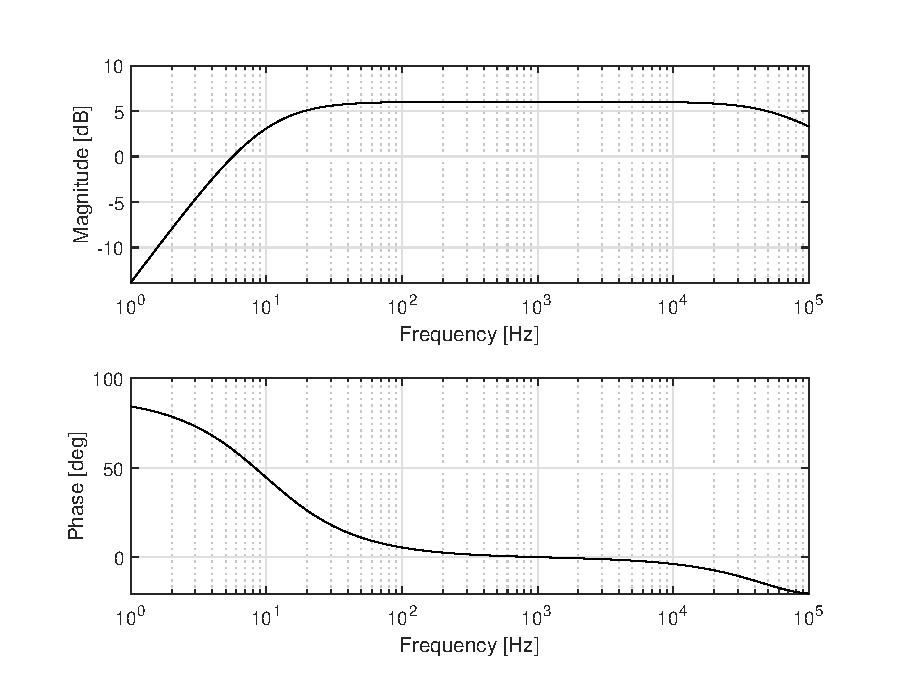
\includegraphics[width=0.6\textwidth]{Synthesis/preamp_input_filter_bode.eps}
	\caption{Bode plot of the designed preamplifier and input filter from a small-signal analysis}
	\label{fig:preamp_input_filter_bode}
\end{figure}

In \autoref{fig:preamp_input_filter_bode} is the bode plot with magnitude and phase. The \SI{6}{\decibel} equal to a gain of 2 is present in the passband. The two cut-off frequencies in \SI{10}{\hertz} and \SI{80}{\kilo\hertz} respectively are also seen.

\section{Modulator}
Based on the original design of the system \cite{multivar_ctrl_loops_for_SM_audio_systems}, the following parameters for the modulator are given by \autoref{tab:design_parameters_modulator}.
\begin{table}[htbp]
	\centering
	\begin{tabular}{@{}llll@{}}
		\toprule
		\multicolumn{1}{c}{\textbf{Name}} & \textbf{Value} & \textbf{Unit} & \textbf{Description} \\ \midrule
		$V_{\mathrm{ref}}$ & $2.5$ & \si{\volt} & Reference voltage \\
		$V_{\mathrm{span}}$ & $2$ & \si{\volt} & Peak-peak maximum input voltage \\
		$V_{\mathrm{hw}}$ & $0.5$  & \si{\volt}  & Hysteresis window \\
		$V_{\mathrm{out}}$ & $5$  & \si{\volt}  & PWM voltage level \\
		$f_{\mathrm{idle}}$ & $600$  & \si{\kilo\hertz}  & Self-oscillating idle frequency \\
		$C$  & $1.5$  & \si{\nano\farad}   & Modulator capacitor \\ \bottomrule
	\end{tabular}
	\caption{Initial design parameters of the modulator}
	\label{tab:design_parameters_modulator}
\end{table}

To determine the $V_{\mathrm{pwm}}$ voltage levels, \Cref{eq:pwm_states_a,eq:pwm_states_b} are used resulting in \Cref{eq:pwm_states_synth_a,eq:pwm_states_synth_b}. 

\begin{subequations} \label{eq:pwm_states_synth}
	\begin{equation} \label{eq:pwm_states_synth_a}
		V_{H} = \frac{V_{\mathrm{out}}}{2} + V_{\mathrm{ref}} = \frac{\SI{5}{\volt}}{2} + \SI{2.5}{\volt} = \SI{5}{\volt}
	\end{equation}
	\begin{equation} \label{eq:pwm_states_synth_b}
		V_{L} = -\frac{V_{\mathrm{out}}}{2} + V_{\mathrm{ref}} = -\frac{\SI{5}{\volt}}{2} + \SI{2.5}{\volt} = \SI{0}{\volt}
	\end{equation}
\end{subequations}

Then the threshold voltages $V_{\mathrm{th}_{H}}$ and $V_{\mathrm{th}_{L}}$ can be calculated from \Cref{eq:hysteresis_window_a,eq:hysteresis_window_b} resulting in \Cref{eq:hysteresis_window_synth_a,eq:hysteresis_window_synth_b}.

\begin{subequations} \label{eq:hysteresis_window_synth}
	\begin{equation} \label{eq:hysteresis_window_synth_a}
		V_{\mathrm{th}_{H}} = V_{\mathrm{hw}} \cdot \frac{V_{H} - V_{\mathrm{ref}}}{V_{H} - V_{L}} + V_{\mathrm{ref}} = \SI{0.5}{\volt} \cdot \frac{\SI{5}{\volt} - \SI{2.5}\volt}{\SI{5}{\volt} - \SI{0}\volt} + \SI{2.5}{\volt} = \SI{2.75}{\volt}
	\end{equation}
	\begin{equation} \label{eq:hysteresis_window_synth_b}
		V_{\mathrm{th}_{L}} = V_{\mathrm{hw}} \cdot \frac{V_{L} - V_{\mathrm{ref}}}{V_{H} - V_{L}} + V_{\mathrm{ref}} = \SI{0.5}{\volt} \cdot \frac{\SI{0}{\volt} - \SI{2.5}\volt}{\SI{5}{\volt} - \SI{0}\volt} + \SI{2.5}{\volt} = \SI{2.25}{\volt}
	\end{equation}
\end{subequations}

Next the carrier waveform voltage limits are calculated from \Cref{eq:carrier_waveform_a,eq:carrier_waveform_b} and results in \Cref{eq:carrier_waveform_synth_a,eq:carrier_waveform_synth_b}. Here an IDLE state is assumed, therefore $V_{\mathrm{in}} = V_{\mathrm{ref}}$.
\begin{subequations} \label{eq:carrier_waveform_synth}
	\begin{equation} \label{eq:carrier_waveform_synth_a}
		\begin{split}
			V_{c_{H}} &= V_{\mathrm{in}} + \frac{V_{\mathrm{span}} \cdot \left( V_{H} - V_{\mathrm{in}} \right) + V_{\mathrm{hw}} \cdot \left( V_{H} - V_{\mathrm{in}} \right)  }{V_{H} - V_{L} + V_{\mathrm{span}}} \\
			&= \SI{2.5}{\volt} + \frac{\SI{2}{\volt} \cdot (\SI{5}{\volt} - \SI{2.5}{\volt}) + \SI{0.5}{\volt} \cdot (\SI{5}{\volt} - \SI{2.5}{\volt})}{\SI{5}{\volt} - \SI{0}{\volt} + \SI{2}{\volt}} \\
			&= \SI{3.393}{\volt}
		\end{split}	
	\end{equation}
	\begin{equation} \label{eq:carrier_waveform_synth_b}
		\begin{split}
				V_{c_{L}} &= V_{\mathrm{in}} + \frac{V_{\mathrm{span}} \cdot \left( V_{L} - V_{\mathrm{in}} \right) + V_{\mathrm{hw}} \cdot \left( V_{L} - V_{\mathrm{in}} \right)  }{V_{H} - V_{L} + V_{\mathrm{span}}} \\
				&= \SI{2.5}{\volt} + \frac{\SI{2}{\volt} \cdot (\SI{0}{\volt} - \SI{2.5}{\volt}) + \SI{0.5}{\volt} \cdot (\SI{0}{\volt} - \SI{2.5}{\volt})}{\SI{5}{\volt} - \SI{0}{\volt} + \SI{2}{\volt}} \\
				&= \SI{1.607}{\volt}
		\end{split}
	\end{equation}
\end{subequations}

The Thevenin resistance as described in \autoref{eq:modulator_thevenin_resistance} results in \autoref{eq:modulator_thevenin_resistance_synth}.

\begin{equation} \label{eq:modulator_thevenin_resistance_synth}
	\begin{split}
		R_{t} &= \frac{1}{f_{\mathrm{idle}} C_{1} \ln{ \left( \frac{(V_{c_{H}} - V_{\mathrm{th}_{L}})(V_{c_{L}} - V_{\mathrm{th}_{H}})}{(V_{c_{H}} - V_{\mathrm{th}_{H}})(V_{c_{L}} - V_{\mathrm{th}_{L}})} \right) }} \\
		&= \frac{1}{\SI{600}{\kilo\hertz} \cdot \SI{1.5}{\nano\farad} \cdot \ln{ \left( \frac{(\SI{3.393}{\volt} - \SI{2.25}{\volt})(\SI{1.607}{\volt} - \SI{2.75}{\volt})}{(\SI{3.393}{\volt} - \SI{2.75}{\volt})(\SI{1.607}{\volt} - \SI{2.25}{\volt})} \right) }} \\
		&= \SI{965.6}{\ohm}
	\end{split}
\end{equation}

In \Cref{eq:modulator_rfb_rin_a,eq:modulator_rfb_rin_b} the expressions for $R_{\mathrm{in}}$ and $R_{\mathrm{fb}}$ were derived. The resulting calculation becomes:

\begin{subequations} \label{eq:modulator_rfb_rin_synth}
	\begin{equation} \label{eq:modulator_rfb_rin_synth_a}
		R_{\mathrm{fb}} = \frac{\SI{2}{\volt} + \SI{5}{\volt}}{\SI{2}{\volt} + \SI{0.5}{\volt}} \cdot \SI{965.6}{\ohm} = \SI{2.704}{\kilo\ohm}
	\end{equation}
	\begin{equation} \label{eq:modulator_rfb_rin_synth_b}
		R_{\mathrm{in}} = \frac{\SI{2.704}{\kilo\ohm} \cdot \SI{965.6}{\ohm}}{\SI{2.704}{\kilo\ohm} + \SI{965.6}{\ohm}} = \SI{1.502}{\kilo\ohm}
	\end{equation}
\end{subequations}

In \Cref{eq:aim_resistor_expression2_a,eq:aim_resistor_expression2_b} the expressions were obtained. It was noted that if one resistor was chosen, the other can be calculated. If value $R_{2} = \SI{20}{\kilo\ohm}$ is chosen the calculation for $R_{1}$ then becomes \Cref{eq:modulator_aim_resistor_synth}.
\begin{equation} \label{eq:modulator_aim_resistor_synth}
	R_{1} = \frac{\SI{0.5}{\volt}}{\SI{5}{\volt} - \SI{0.5}{\volt}} \cdot \SI{20}{\kilo\ohm} = \SI{2.22}{\kilo\ohm}
\end{equation}

The chosen $V_{\mathrm{hw}} = \SI{0.5}{\volt}$ is a relatively minor hysteresis window in a DR of \SI{5}{\volt}. The benefit is a more linear transfer function \cite{multivar_ctrl_loops_for_SM_audio_systems}. Implementing the calculations above, a prediction can be calculated of the behavior of the self-oscillating characteristic of the AIM modulator.

\begin{figure}[htbp]
	\centering
	\begin{subfigure}[t]{0.4\textwidth}
		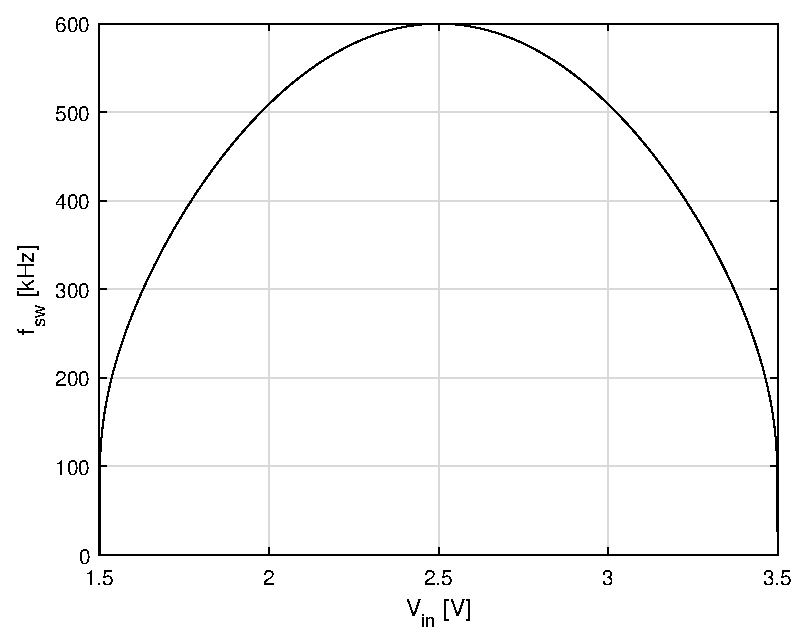
\includegraphics[width=0.9\linewidth]{Synthesis/modulator_fsw.eps}
		\subcaption{$f_{\mathrm{sw}}$ over $V_{\mathrm{in}}$}
		\label{fig:modulator_fsw_synth}
	\end{subfigure}%
	\begin{subfigure}[t]{0.4\textwidth}
		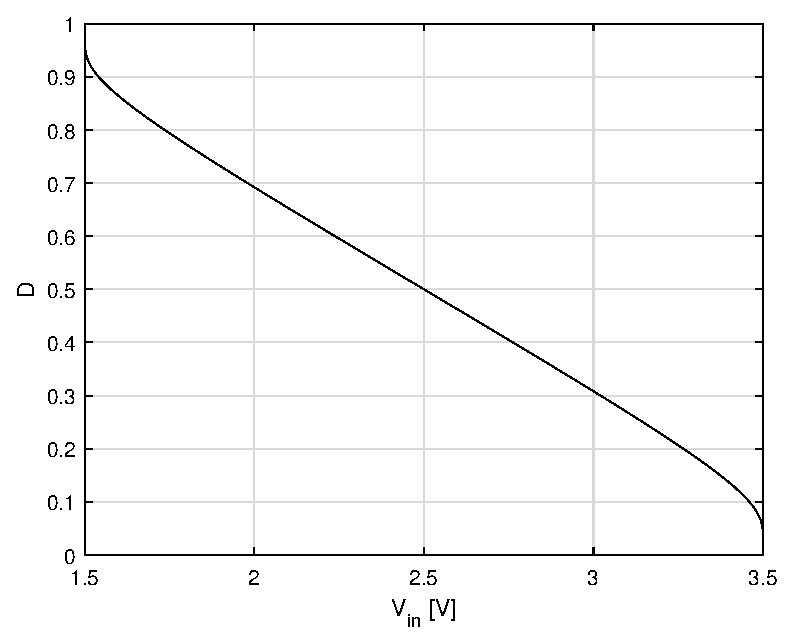
\includegraphics[width=0.9\linewidth]{Synthesis/modulator_duty.eps}
		\subcaption{$D$ over $V_{\mathrm{in}}$}
		\label{fig:modulator_duty_synth}
	\end{subfigure}
	\caption{Calculated $f_{\mathrm{sw}}$ and $D$ over different DC levels of $V_{\mathrm{in}}$}
	\label{fig:modulator_fsw_duty_synth}
\end{figure}

Seen in \Cref{fig:modulator_fsw_synth}, the idle frequency is determined as the vertex point of the arc shape at \SI{600}{\kilo\hertz}. This is in agreement with the initial design specifications. There is a symmetrical roll-off when $V_{\mathrm{in}}$ deviates to either side within $V_{\mathrm{span}}$. Looking at \Cref{fig:modulator_duty_synth}, if $V_{\mathrm{in}}$ is outside the operating region of $V_{\mathrm{ref}}\pm\frac{V_{\mathrm{span}}}{2}=\SI{2.5}{\volt}\pm\SI{1}{\volt}$, the duty cycle becomes either \SI{0}{\percent} or \SI{100}{\percent}, resulting in modulator clipping. 

\section{Gate Driver}
In the reference design, the capacitive components were specified to be \SI{100}{\pico\farad}. That means the remaining unknown variable is the resistive component in the RC-network. As this is a variable resistor, it will have to be carefully tuned once the amplifier is produced.

\section{Power Stage}
In the full-bridge output configuration of the class-D amplifier, there will be a $\SI{30}{\volt}$ DC supply. The N-channel BSZ097N10NS5 \cite{BSZ097N10NS5} MOSFET is used as a switching device for $Q_{1}$, $Q_{2}$, $Q_{3}$ and $Q_{4}$. The component is from the original design \cite{nagy_special_course}, and is a good fit in cost-effectiveness, and has robust specifications for this application.

\section{Output Filter}
For the output filter, the design method is also based on the previous design \cite{nagy_special_course}. The output LPF cut-off frequency is designated as 
\begin{equation}
	f_{n} = f_{c} = \frac{1}{10} \cdot f_{\mathrm{idle}} = \frac{1}{10} \cdot \SI{600}{\kilo\hertz} = \SI{60}{\kilo\hertz}
\end{equation}

That puts its $\SI{-3}{\decibel}$ cut-off point a decade below the modulation frequency in the spectrum and follows the convention of the previous design \cite{multivar_ctrl_loops_for_SM_audio_systems}. The initial design parameters can be seen in \autoref{tab:design_parameters_power_stage}.

\begin{table}[htbp]
	\centering
	\begin{tabular}{@{}llll@{}}
		\toprule
		\multicolumn{1}{c}{\textbf{Name}} & \textbf{Value} & \textbf{Unit} & \textbf{Description} \\ \midrule
		$f_{n}$ & $60$ & \si{\kilo\hertz} & Low-pass filter natural frequency \\
		%$\zeta$ & $0.316$ & \si{1} & Damping ratio \\
		$Q$ & $3$  & \si{1}  & Quality factor \\
		$R_{\mathrm{BTL}}$ & $4$  & \si{\ohm}  & Bridge-tied load \\
		$V_{\mathrm{DD}}$ & $30$  & \si{\volt}  & Power supply voltage \\
		%$P_{\mathrm{max}}$  & $110$  & \si{\watt}   & Maximum average power \\ 
		\bottomrule
	\end{tabular}
	\caption{Initial design parameters of the power stage}
	\label{tab:design_parameters_power_stage}
\end{table}

The Q value is a chosen and somewhat arbitrary value that is required before the component selection can be initiated. Although based on previous stipulations of desired resonance, a rather high value is chosen. According to \autoref{eq:q_factor_zeta}, with the chosen Q factor of the filter, the damping ratio would thus become:

\begin{equation} \label{eq:zeta_synth}
	\zeta = \frac{1}{2Q} = 0.167
\end{equation}

To design the output filter and obtain its component values, the single-ended load must be determined. According to \Cref{eq:r_f_btl}, the transformation expression is:
\begin{equation} \label{eq:output_filter_rf_synth}
	R_{f} = \frac{\SI{4}{\ohm}}{2} = \SI{2}{\ohm}
\end{equation}

Now that the equivalent single-ended load is determined, the two output filter reactive elements for the single-ended configuration can be calculated. From \Cref{eq:output_filter_l_ind,eq:output_filter_c_f} the calculation becomes:
\begin{subequations} \label{eq:output_filter_synth}
	\begin{equation} \label{eq:output_filter_l_ind_synth}
		L_{\mathrm{ind}} = \frac{\SI{2}{\ohm}}{2\pi \cdot 3 \cdot \SI{60}{\kilo\hertz}} = \SI{1.768}{\micro\henry}
	\end{equation}
	\begin{equation} \label{eq:output_filter_c_f_synth}
		C_{f} = \frac{3}{2\pi \cdot \SI{60}{\kilo\hertz} \cdot \SI{2}{\ohm}} = \SI{3.96}{\micro\farad}
	\end{equation}
\end{subequations}

Now the single-ended capacitor $C_{f}$ is transformed back into the differential capacitor $C_{\mathrm{BTL}}$ according to \autoref{eq:c_f_btl} and the straightforward calculation becomes:
\begin{equation} \label{eq:c_f_btl_synth}
	C_{\mathrm{BTL}} = \frac{\SI{3.96}{\micro\farad}}{2} = \SI{1.98}{\micro\farad}
\end{equation}

%\begin{figure}[H]
%	\centering
%	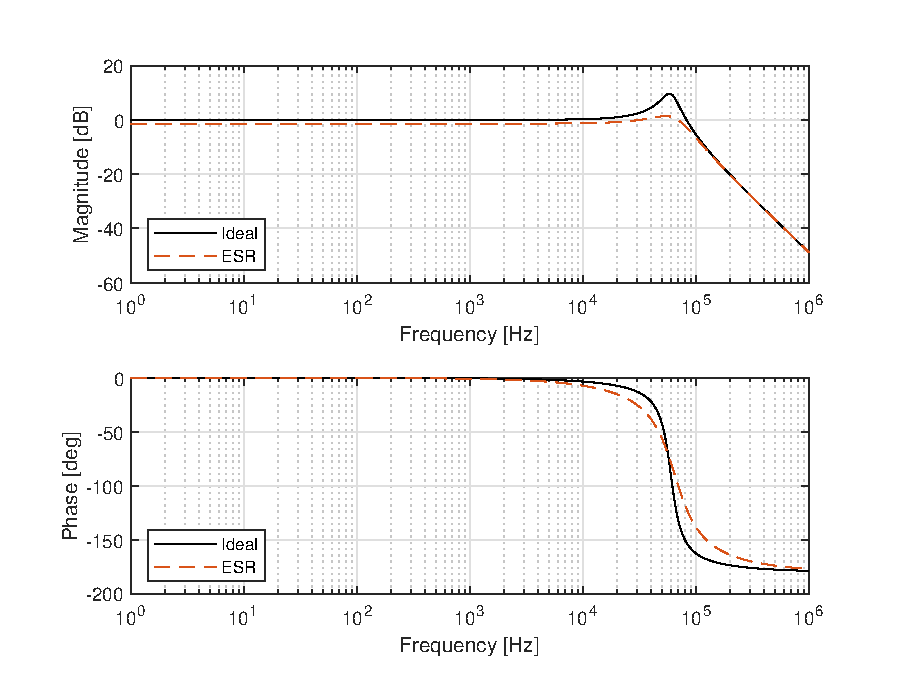
\includegraphics[width=0.9\textwidth]{Synthesis/output_filter_bode.eps}
%	\caption{Bode plot of the designed output filter from a small-signal analysis}
%	\label{fig:output_filter_bode}
%\end{figure}
%
%Using the synthesized values, a bode plot is seen in \autoref{fig:output_filter_bode} using ideal component values and an estimated ESR of \SI{350}{\milli\ohm} using stipulations in \cite{multivar_ctrl_loops_for_SM_audio_systems} is modelled by \autoref{fig:ltspice_output_filter}. It is seen that the ESR of the inductor significantly reduces the peak of the 

Now the single-ended output filter components have been calculated and transformed into differential output filter components that can be applied in the circuit.

\section{Reference Voltage}
In the section explaining the theory of this subcircuit, it was specified that the cathode node current should be between \SIrange{0.1}{15}{\milli\ampere}. An insufficient or excessive node current is outside the operating ranges of the shunt regulator. Therefore, a \SI{2}{\milli\ampere} node current is chosen. Using Ohm's law, we have:
\begin{equation}
	R_{\mathrm{sup}} = \frac{V_{s}}{I_{\mathrm{sup}}} = \frac{\SI{5}{\volt}}{\SI{2}{\milli\ampere}} = \SI{2.5}{\kilo\ohm}
\end{equation}

The reference voltage is then determined by its two resistors $R_{\mathrm{A1}}$ and $R_{\mathrm{A2}}$ in a voltage divider configuration. Referring to the theory section on this subcircuit, where $V_{\mathrm{ref}_{\mathrm{IC}}} = \SI{1.24}{\volt}$ according to the datasheet, and $R_{\mathrm{A1}} = \SI{4.75}{\kilo\ohm}$ is chosen, we calculate by rewriting \autoref{eq:reference_voltage} and the calculation becomes:
\begin{equation} \label{eq:reference_voltage_synth}
	R_{\mathrm{A2}} = \frac{V_{\mathrm{ref}_{\mathrm{IC}}} \cdot R_{\mathrm{A1}}}{V_{\mathrm{ref}} - V_{\mathrm{ref}_{\mathrm{IC}}}} = \frac{\SI{1.24}{\volt} \cdot \SI{5}{\kilo\ohm}}{\SI{2.5}{\volt} - \SI{1.24}{\volt}} = \SI{4.92}{\kilo\ohm}
\end{equation}
Now the numeric values of both resistors have been determined as $R_{\mathrm{A1}} = \SI{5}{\kilo\ohm}$ and $R_{\mathrm{A2}} = \SI{4.68}{\kilo\ohm}$. This appears logical, as the resistors are placed in a voltage divider configuration. The two resistances are practically equivalent, and as half of the supply voltage is desired it conforms well with the fundamental principles of electric circuits. In practice, they will possess an equal value.
In the PCB reference notation, the components are $R_{\mathrm{A1}} = R_{4}$ and $R_{\mathrm{A2}} = R_{7}$.

\section{Regulation and Control}
As mentioned in the theory section of the regulation and control there are a PI controller and an LQR present in the system. The synthesis process will be explained in this section and the initial design parameters described in the table below:
\begin{table}[htbp]
	\centering
	\begin{tabular}{@{}llll@{}}
		\toprule
		\multicolumn{1}{c}{\textbf{Name}} & \textbf{Value} & \textbf{Unit} & \textbf{Description} \\ \midrule
		$C_{\mathrm{BTL}}$ & $1.98$ & \si{\micro\farad} & Output filter capacitance \\
		$L_{\mathrm{ind}}$ & $1.768$ & \si{\micro\henry} & Output filter inductance \\
		$R_{\mathrm{ind}}$ & $15$  & \si{\milli\ohm}  & Output filter shunt \\
		$R_{\mathrm{BTL}}$ & $4$  & \si{\ohm}  & Bridge-tied load \\
		$R_{\mathrm{in}}$ & $1.5$  & \si{\kilo\ohm}  & Modulator input resistance \\ 
		$\mathrm{Gain}$ & $25$ & \si{1} & Amplifier gain \\ \bottomrule
	\end{tabular}
	\caption{Initial design parameters of the regulator}
	\label{tab:design_parameters_regulator}
\end{table}

The PI regulator is synthesised based on an initial chosen variable and hand-tuning it based on the result of the expressions. First the filter component values are transformed to single-ended, based on \Cref{eq:output_filter_rf_synth,eq:output_filter_c_f_synth}, yields:
$$R_{f} = \SI{2}{\ohm}$$
$$C_{f} = \SI{3.96}{\micro\farad}$$

Through some hand-tuning, the following coefficients were chosen for the regulator synthesis:
$$K_{i} = \num{2e3}$$
$$\mathrm{gu} = \pi$$

And then using MATLAB R2020a with the Control System Toolbox \cite{matlab_control_toolbox}, with the following state space model comprised of an input matrix $B$, system matrix $A$ and output matrix $C$ from the ODE in \cite{multivar_ctrl_loops_for_SM_audio_systems}:
\begin{subequations}
	\begin{equation}
		A = \begin{bmatrix}	-\frac{R_{\mathrm{ind}}}{L_{\mathrm{ind}}} & -\frac{1}{L_{\mathrm{ind}}} \\ \frac{1}{C_{f}} & -\frac{1}{C_{f}\cdot R_{f}} \end{bmatrix} = \begin{bmatrix} -8.482E3 & -5.655E5 \\ 2.525E5 & 1.263E5 \end{bmatrix}
	\end{equation}	
	\begin{equation}
		B = \begin{bmatrix} \frac{Gain}{L_{\mathrm{ind}}} \\ 0 \end{bmatrix} = \begin{bmatrix} 1.244E7 \\ 0 \end{bmatrix}
	\end{equation}
	\begin{equation}
		C = \begin{bmatrix} 0 & 1 \end{bmatrix}
	\end{equation}
	\begin{equation}
		G = ss \left( A, B, \begin{bmatrix} C \\ zeros(2) \end{bmatrix}, 0 \right) 
	\end{equation}
\end{subequations} 

With some further matrix augmentation and calculation the regulator calculation, in accordance with \autoref{lst:lqi_designer}, yielding the following parameters for the PI controller:
\begin{subequations}
	\begin{equation}
		C_{\mathrm{PI}} = \SI{1.5}{\nano\farad}
	\end{equation}
	\begin{equation}
		R_{\mathrm{PI}} = \SI{33.3}{\kilo\ohm}
	\end{equation}
\end{subequations}
Where $C_{\mathrm{PI}} = C_{14}$ and $R_{\mathrm{PI}}=R_{5}$. And for the LQR:
\begin{subequations}
	\begin{equation}
		R_{k_{1}} = \SI{16.2}{\kilo\ohm}
	\end{equation}
	\begin{equation}
		R_{k_{2}} = \SI{8.63}{\kilo\ohm}
	\end{equation}
\end{subequations}
Where $R_{k_{1}}=R_{18}$ and $R_{k_{2}}=R_{14}$. Now the values for the discrete analogue components in the PI controller and the LQR have been determined.

\begin{figure}[htbp]
	\centering
	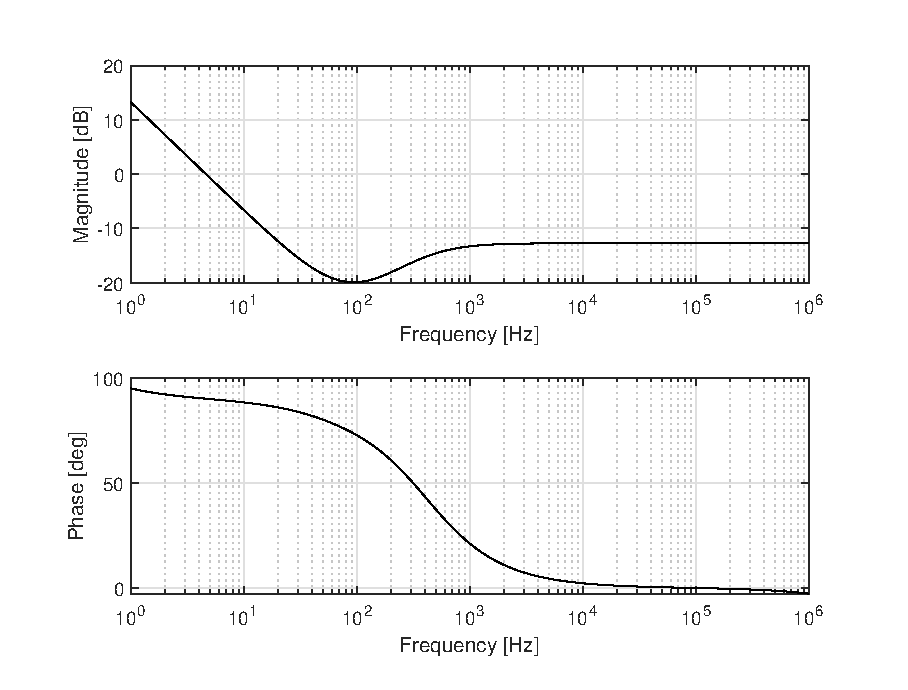
\includegraphics[width=0.6\textwidth]{Synthesis/pi_controller_bode.eps}
	\caption{Bode plot of the designed PI controller from a small-signal analysis}
	\label{fig:pi_controller_bode}
\end{figure}

Applying the synthesized values, a bode plot is seen in \autoref{fig:pi_controller_bode} where the steady-state integrator is present. In the upper subfigure, the magnitude is shown in \si{\decibel} and in the lower subfigure, the phase is shown in degrees. The small-signal analysis that was used to obtain the bode plot above can be found in \autoref{fig:ltspice_pi_regulator_ac}.

\section{Remarks}
This concludes the synthesis chapter of the report. The entire BOM based on Synthesis chapter can be found in the appendix on \autoref{tab:bom}. During the production phase, some modifications were made to the design, which will be explained in the following chapter.